\documentclass[10.5pt,letterpaper]{article}

% --- Typography & Layout (Google DeepMind Technical Report Style) ---
\usepackage[LSBC4,T1]{fontenc}
\usepackage[utf8]{inputenc}
\usepackage[default,regular,semibold]{sourcesanspro}
\usepackage{microtype}
\usepackage[left=0.95in,right=0.95in,top=0.92in,bottom=0.92in]{geometry}
\usepackage{amsmath,amssymb}
\usepackage{booktabs}
\usepackage{tabularx}
\usepackage{xcolor}
\usepackage{hyperref}
\usepackage{fancyhdr}
\usepackage[nobottomtitles*]{titlesec}
\renewcommand{\bottomtitlespace}{.14\textheight}
\usepackage{listings}
\usepackage{tikz}
\usepackage{pgfplots}
\usepackage{caption}
\usepackage{float}
\usepackage{enumitem}
\usepackage{xurl}
\usepackage{chessboard}
\usepackage[most]{tcolorbox}

\sloppy
\pgfplotsset{compat=1.18}
\usetikzlibrary{arrows.meta,positioning,shapes.geometric}

% --- DeepMind Color Palette ---
\definecolor{dmblue}{RGB}{26,115,232}
\definecolor{dmnavy}{RGB}{15,23,42}
\definecolor{dmslate}{RGB}{71,85,105}
\definecolor{dmmuted}{RGB}{100,116,139}
\definecolor{dmteal}{RGB}{13,148,136}
\definecolor{dmcoral}{RGB}{225,29,72}
\definecolor{dmamber}{RGB}{217,119,6}
\definecolor{dmpurple}{RGB}{124,58,237}
\definecolor{dmbg}{RGB}{244,247,252}
\definecolor{dmcard}{RGB}{248,250,252}
\definecolor{dmborder}{RGB}{226,232,240}
\definecolor{dmgoodbg}{RGB}{240,253,244}
\definecolor{dmbadbg}{RGB}{255,241,242}
\definecolor{boardlight}{RGB}{248,250,252}
\definecolor{boarddark}{RGB}{186,198,214}
\definecolor{boardframe}{RGB}{100,116,139}

% --- Spacing & Paragraph Rhythm ---
\linespread{1.15}
\setlength{\parindent}{0pt}
\setlength{\parskip}{5.5pt}
\setlist[itemize]{leftmargin=1.3em, itemsep=3pt, topsep=3pt}
\setlist[enumerate]{leftmargin=1.5em, itemsep=3pt, topsep=3pt}

% --- Headings (Clean Sans-Serif Hierarchy) ---
\titleformat{\section}
  {\Large\bfseries\color{dmnavy}}
  {\textcolor{dmblue}{\thesection}}{0.75em}{}
  [\vspace{2pt}{\color{dmborder}\titlerule[0.8pt]}]
\titlespacing*{\section}{0pt}{16pt}{7pt}

\titleformat{\subsection}
  {\large\bfseries\color{dmnavy}}
  {\textcolor{dmslate}{\thesubsection}}{0.6em}{}
\titlespacing*{\subsection}{0pt}{12pt}{4pt}

\titleformat{\paragraph}[runin]
  {\bfseries\color{dmnavy}}{}{0pt}{}[.\;\;]

% --- Header & Footer ---
\pagestyle{fancy}
\fancyhf{}
\renewcommand{\headrulewidth}{0.4pt}
\renewcommand{\headrule}{\hbox to\headwidth{\color{dmborder}\leaders\hrule height \headrulewidth\hfill}}
\fancyhead[L]{\footnotesize\color{dmmuted}\nouppercase{\leftmark}}
\fancyhead[R]{\footnotesize\color{dmmuted}\textbf{Chatarunga} Technical Report}
\fancyfoot[C]{\footnotesize\color{dmmuted}\thepage}

% --- Hyperlinks ---
\hypersetup{
    colorlinks=true,
    linkcolor=dmblue,
    citecolor=dmblue,
    urlcolor=dmblue,
    pdftitle={Chatarunga: From Scratch to Beating Stockfish 18 in Zero-Dependency Rust},
    pdfauthor={Deedy Das (USA)}
}

% --- Captions ---
\captionsetup{
    font={small,color=dmslate},
    labelfont={bf,color=dmnavy},
    skip=6pt
}

% --- DeepMind Callout Boxes ---
\newtcolorbox{abstractbox}{
    colback=dmbg,
    colframe=dmbg,
    borderline west={3pt}{0pt}{dmblue},
    boxrule=0pt,
    arc=2pt,
    left=12pt, right=12pt, top=10pt, bottom=10pt,
    breakable
}

\newtcolorbox{takeawaybox}[1][Key Takeaway]{
    colback=dmgoodbg,
    colframe=dmteal!35,
    borderline west={3pt}{0pt}{dmteal},
    boxrule=0.4pt,
    arc=3pt,
    left=10pt, right=10pt, top=7pt, bottom=7pt,
    title={\small\bfseries\color{dmteal!80!black}#1},
    coltitle=dmnavy,
    attach title to upper={\par\vspace{2pt}},
    breakable
}

\newtcolorbox{failurebox}[1][What Broke --- And Why]{
    colback=dmbadbg,
    colframe=dmcoral!30,
    borderline west={3pt}{0pt}{dmcoral},
    boxrule=0.4pt,
    arc=3pt,
    left=10pt, right=10pt, top=7pt, bottom=7pt,
    title={\small\bfseries\color{dmcoral!85!black}#1},
    coltitle=dmnavy,
    attach title to upper={\par\vspace{2pt}},
    breakable
}

\newtcolorbox{insightbox}[1][Design Insight]{
    colback=dmbg,
    colframe=dmblue!25,
    borderline west={3pt}{0pt}{dmblue},
    boxrule=0.4pt,
    arc=3pt,
    left=10pt, right=10pt, top=7pt, bottom=7pt,
    title={\small\bfseries\color{dmblue!85!black}#1},
    coltitle=dmnavy,
    attach title to upper={\par\vspace{2pt}},
    breakable
}

% --- Colored Chessboard Defaults (Clean Modern Slate & White Theme) ---
\setchessboard{
    smallboard,
    showmover=true,
    moverstyle=triangle,
    labelleft=true,
    labelbottom=true,
    boardfontencoding=LSBC4,
    setfontcolors,
    whitefieldmaskcolor=boardlight,
    blackfieldmaskcolor=boarddark,
    whitepiececolor=black,
    whiteonwhitepiecemaskcolor=white,
    whiteonblackpiecemaskcolor=white,
    blackpiececolor=black,
    blackonwhitepiecemaskcolor=black,
    blackonblackpiecemaskcolor=black,
    borderwidth=0.9pt,
    bordercolor=boardframe,
    pgfstyle=straightmove,
    linewidth=0.16em,
    arrow=to,
}

% --- Code Listings (Used in Technical Appendix Only) ---
\lstdefinelanguage{Rust}{
    morekeywords={fn,let,mut,pub,struct,impl,enum,match,if,else,for,while,loop,return,use,const,unsafe,as,in,ref,where,Self,self,true,false,usize,u8,u16,u32,u64,i8,i16,i32,i64,f32,f64,bool,Option,Some,None,Vec,Arc,Box},
    sensitive=true,
    morecomment=[l]{//},
    morecomment=[s]{/*}{*/},
    morestring=[b]",
}
\lstset{
    basicstyle=\ttfamily\scriptsize,
    backgroundcolor=\color{dmcard},
    frame=single,
    rulecolor=\color{dmborder},
    keywordstyle=\color{dmblue}\bfseries,
    commentstyle=\color{dmmuted}\itshape,
    stringstyle=\color{dmteal},
    numbers=left,
    numberstyle=\tiny\color{dmmuted},
    numbersep=7pt,
    tabsize=4,
    breaklines=true,
    showstringspaces=false,
    xleftmargin=10pt,
    framexleftmargin=8pt,
    aboveskip=6pt,
    belowskip=6pt,
}

% ==============================================================================
\begin{document}
\thispagestyle{empty}

% --- DeepMind-Style Title Header ---
{\color{dmblue}\rule{\textwidth}{2.6pt}}\par\vspace{10pt}
{\footnotesize\bfseries\color{dmblue} TECHNICAL REPORT \quad$\cdot$\quad OPEN-SOURCE CHESS AI SYSTEMS \quad$\cdot$\quad NOVEMBER 2026}\par\vspace{6pt}
{\fontsize{22}{27}\selectfont\bfseries\color{dmnavy} Chatarunga:\\
From Scratch to Beating Stockfish~18 in Zero-Dependency Rust}\par\vspace{8pt}
{\normalsize\color{dmslate} \textbf{Deedy Das (USA)} \quad$\cdot$\quad MIT License \quad$\cdot$\quad \href{https://github.com/deedy/chess-chatarunga}{\texttt{github.com/deedy/chess-chatarunga}}}\\
{\small\color{dmmuted} Cross-Platform AVX2 / ARM64 NEON UCI Engine \quad$\cdot$\quad Apple M5~Max \& Modal NVIDIA H100/H200 GPUs}\par\vspace{12pt}

% --- Shaded Abstract Card ---
\begin{abstractbox}
\textbf{\color{dmnavy}Abstract.}\;
Modern superhuman chess engines pair blazingly fast board manipulation, deeply selective alpha-beta search, and compact neural networks that evaluate millions of positions per second on an ordinary CPU. Yet most engine descriptions present only the finished release, omitting the calibration bugs, over-pruning regressions, and cache-bandwidth laws that determine real playing strength. In this report, we present \textbf{Chatarunga}---an open-source, zero-dependency Rust UCI chess engine built from an empty directory---and document its complete \textbf{+860+~Elo} climb from a 2,660-Elo hand-crafted baseline through \textbf{Chatarunga~1.0} and \textbf{Chatarunga~2.0} (with a live preview of \textbf{Search~v8}).

On a single CPU core, \textbf{Chatarunga~2.0} reaches \textbf{$\approx 3{,}440\text{--}3{,}480$~CCRL} ($\sim$\#95--\#110 overall), overtaking CCRL~\#98 \texttt{akimbo 1.1.0-dev} head-to-head (\textbf{$+12 =37 -11$, 50.83\%}, zero lost pairs---a $+94.5$~Elo jump over Chatarunga~1.0). Scaling to \textbf{4~CPU cores via Lazy SMP}, Chatarunga~2.0 reaches \textbf{$\approx 3{,}521 \pm 64$~CCRL} ($\sim$\#75--\#79 on live CCRL~40/15), scoring \textbf{35.00\% ($+7 =28 -25$, 7~decisive checkmate wins and 3~won pairs)} against unthrottled \textbf{Stockfish~18 (1CPU = 3,628~CCRL)}---up from a single win in Chatarunga~1.0. Our latest \textbf{Search~v8} engine adds a further \textbf{$+43.7 \pm 31.0$~Elo} (LOS~99.7\%, zero lost pairs) over Chatarunga~2.0 on the exact same neural network, lifting 4-CPU Stockfish~18 score to \textbf{36.67\% ($+4 =36 -20$, only 1~lost pair, $\approx 3{,}533 \pm 45$~CCRL)} and beating CCRL~\#47 \texttt{Velvet 8.1.1} on both 1~and 4~threads, while a direct 1-CPU test against CCRL~\#51 \texttt{Motor 0.9.0} (3,570) sets an honest conservative single-core floor ($\approx 3{,}436 \pm 62$, consensus \textbf{$\approx 3{,}460\text{--}3{,}520$~1-CPU / $\approx 3{,}535\text{--}3{,}570$~4-CPU}).

Along the way, we report eight concrete empirical lessons: (1)~small bugs in evaluation scale headers, parallel thread voting, and Windows 1~MB stack limits can silently destroy 100--450~Elo or crash production binaries; (2)~joint 25- to 38-parameter SPSA tuning delivered $+184$~Elo in a single pass; (3)~across 6.0~billion training steps in global H200 VRAM, \textbf{SCReLU beats Pairwise-CReLU by $+44$ to $+60$~Elo} in real search even when Pairwise has lower validation MSE; (4)~an \textbf{L2/SLC Cache-Residency Law} governs wall-clock strength, allowing a compact 25.2~MB $16\times 1024$ SCReLU network (1.68M~nps) to beat wider $16\times 1536$ and $32\times 1536$ networks by $+22$ to $+74$~Elo on the clock; (5)~blindly extending pruning depths without SPSA cost $-35$~Elo; (6)~\textbf{UHO overfitting and un-rescored Lc0 data traps}---mixing unbalanced UHO data gained $+43.7$~Elo on UHO yet regressed $-39$~Elo on balanced ECO against Stockfish~18, while un-rescored Lc0~T80 lost $-115$~Elo; (7)~our neural networks organically rediscovered grandmaster piece values and fortress theory, while explicit threat inputs doubled depth-0 hanging-piece awareness; and (8)~multi-rival 1-CPU and 4-CPU calibration against Stockfish~18, \texttt{Motor 0.9.0}, \texttt{Velvet 8.1.1}, and \texttt{akimbo}---including auditing opponent \texttt{movetime} compliance---gives an honest, reproducible map to CCRL Top~50.
\end{abstractbox}

\vspace{6pt}
\begin{center}
\small
\begin{tabular}{@{}l@{\quad\;\;}l@{\quad\;\;}l@{\quad\;\;}l@{}}
\textbf{\color{dmnavy}Search v8 (1-CPU)} & \textbf{\color{dmnavy}Search v8 (4-CPU)} & \textbf{\color{dmnavy}vs.\ Stockfish 18 (4T vs 1T)} & \textbf{\color{dmnavy}v1 $\to$ v2 $\to$ Search v8} \\
\color{dmblue}\textbf{$\approx 3{,}460\text{--}3{,}520$~CCRL} & \color{dmblue}\textbf{$\approx 3{,}535\text{--}3{,}570$~CCRL} & \color{dmteal}\textbf{36.7\% (v8) / 7 wins (v2)} & \color{dmteal}\textbf{$+76.5$ / $+43.7$~Elo} \\
\end{tabular}
\end{center}
\vspace{2pt}
{\color{dmborder}\rule{\textwidth}{0.6pt}}

% ==============================================================================
\section{The Climb: From 2,660 Elo to Seven Wins Over Stockfish 18}
% ==============================================================================

Named after \emph{Chaturanga}---the sixth-century Indian ancestor of modern chess---\textbf{Chatarunga} began as an empty Rust workspace with a strict engineering constraint: \textbf{zero external Cargo dependencies}.\footnote{Written in Rust~1.94.0 with an empty \texttt{[dependencies]} table in \texttt{Cargo.toml} (\href{https://github.com/deedy/chess-chatarunga}{\texttt{github.com/deedy/chess-chatarunga}}). All local matches ran on an Apple M5~Max (18~CPU cores, ARMv8.6-A NEON + \texttt{dotprod}); multi-platform x86-64 AVX2, x86-64 POPCNT, Linux, and macOS binaries are CI-verified via GitHub Actions; large-scale neural training ran on Modal NVIDIA H100/H200 GPUs. Every score, Elo interval, and game in this report is backed verbatim by logs in \texttt{chess/logs/}.} Our goal was to answer a direct question: \emph{how close can a clean, transparent, single-author engine get to Stockfish~18 and the global CCRL Top~50, and what actually separates a 3,400 engine from a 3,570+ engine?}

Over eight search generations and two public releases (\textbf{Chatarunga~1.0} and \textbf{Chatarunga~2.0}), playing strength climbed by \textbf{nearly +900~Elo}: passing grandmaster level ($\approx 2{,}840$) via \emph{100\% pure self-play}, breaking Stockfish~18's \texttt{UCI\_Elo=3190} cap on a single core, scoring our first checkmate victory over unthrottled Stockfish~18 in \textbf{Chatarunga~1.0} (4-CPU, $\approx 3{,}467$~CCRL), jumping \textbf{$+76.5$~Elo} in \textbf{Chatarunga~2.0} to overtake CCRL~\#98 \texttt{akimbo} on \textbf{1-CPU} ($\approx 3{,}480$~CCRL) while scoring \textbf{7~wins (35.0\%)} against Stockfish~18 on \textbf{4-CPU} ($\approx 3{,}521$~CCRL), and gaining another \textbf{$+43.7$~Elo} in our current \textbf{Search~v8} engine.

\begin{figure}[H]
\centering
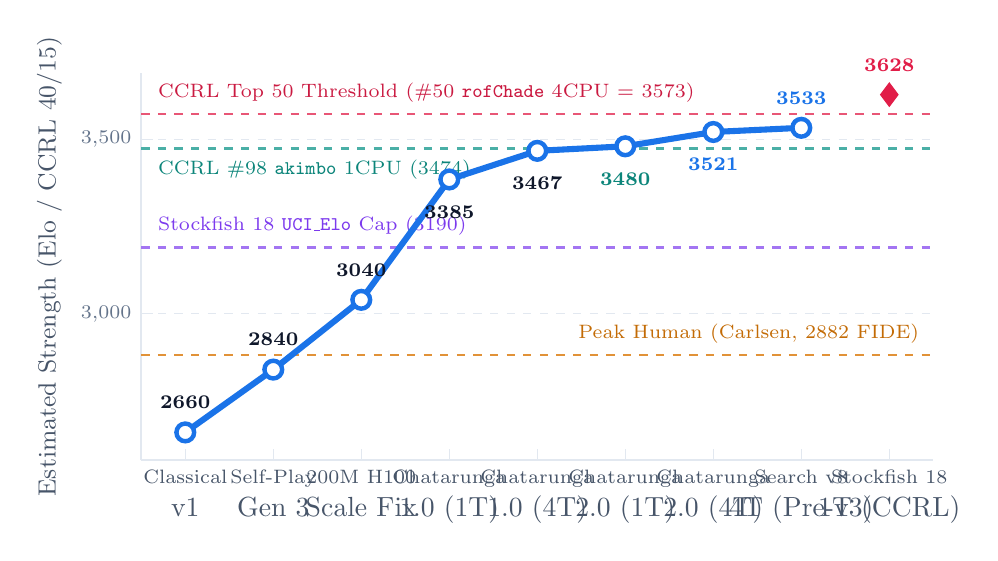
\begin{tikzpicture}
\begin{axis}[
    width=0.96\textwidth,
    height=6.5cm,
    axis x line*=bottom,
    axis y line*=left,
    axis line style={dmborder, line width=0.8pt},
    tick style={dmborder},
    ylabel={\small\color{dmslate}Estimated Strength (Elo / CCRL 40/15)},
    ymin=2580, ymax=3690,
    xmin=0.5, xmax=9.5,
    xtick={1,2,3,4,5,6,7,8,9},
    xticklabels={
        {\scriptsize Classical\\v1},
        {\scriptsize Self-Play\\Gen~3},
        {\scriptsize 200M H100\\Scale Fix},
        {\scriptsize Chatarunga\\1.0 (1T)},
        {\scriptsize Chatarunga\\1.0 (4T)},
        {\scriptsize Chatarunga\\2.0 (1T)},
        {\scriptsize Chatarunga\\2.0 (4T)},
        {\scriptsize Search v8\\4T (Pre-v3)},
        {\scriptsize Stockfish 18\\1T (CCRL)}
    },
    xticklabel style={align=center, color=dmslate},
    yticklabel style={font=\scriptsize, color=dmmuted},
    ymajorgrids=true,
    grid style={dashed, dmborder},
    clip=false,
]
% Reference lines
\draw[dashed, dmamber!80, line width=0.85pt] (axis cs:0.5,2882) -- (axis cs:9.5,2882);
\node[font=\scriptsize, anchor=south east, color=dmamber!90!black] at (axis cs:9.45,2888) {Peak Human (Carlsen, 2882 FIDE)};

\draw[dashed, dmpurple!70, line width=0.85pt] (axis cs:0.5,3190) -- (axis cs:9.5,3190);
\node[font=\scriptsize, anchor=south west, color=dmpurple] at (axis cs:0.58,3196) {Stockfish 18 \texttt{UCI\_Elo} Cap (3190)};

\draw[dashed, dmteal!75, line width=0.85pt] (axis cs:0.5,3474) -- (axis cs:9.5,3474);
\node[font=\scriptsize, anchor=north west, color=dmteal!90!black] at (axis cs:0.58,3468) {CCRL \#98 \texttt{akimbo} 1CPU (3474)};

\draw[dashed, dmcoral!75, line width=0.85pt] (axis cs:0.5,3573) -- (axis cs:9.5,3573);
\node[font=\scriptsize, anchor=south west, color=dmcoral!90!black] at (axis cs:0.58,3579) {CCRL Top 50 Threshold (\#50 \texttt{rofChade} 4CPU = 3573)};

% Progression curve (1-CPU + 4-CPU milestones)
\addplot[color=dmblue, line width=2.2pt, mark=*, mark size=3.2pt, mark options={fill=white, draw=dmblue, line width=1.6pt}] coordinates {
    (1,2660) (2,2840) (3,3040) (4,3385) (5,3467) (6,3480) (7,3521) (8,3533)
};
% Stockfish 18 reference point
\addplot[only marks, mark=diamond*, mark size=4.2pt, color=dmcoral] coordinates {(9,3628)};

% Value labels
\node[font=\scriptsize\bfseries, color=dmnavy, above=5pt] at (axis cs:1,2660) {2660};
\node[font=\scriptsize\bfseries, color=dmnavy, above=5pt] at (axis cs:2,2840) {2840};
\node[font=\scriptsize\bfseries, color=dmnavy, above=5pt] at (axis cs:3,3040) {3040};
\node[font=\scriptsize\bfseries, color=dmnavy, below=6pt] at (axis cs:4,3385) {3385};
\node[font=\scriptsize\bfseries, color=dmnavy, below=6pt] at (axis cs:5,3467) {3467};
\node[font=\scriptsize\bfseries, color=dmteal!90!black, below=6pt] at (axis cs:6,3480) {3480};
\node[font=\scriptsize\bfseries, color=dmblue, below=6pt] at (axis cs:7,3521) {3521};
\node[font=\scriptsize\bfseries, color=dmblue, above=5pt] at (axis cs:8,3533) {3533};
\node[font=\scriptsize\bfseries, color=dmcoral, above=5pt] at (axis cs:9,3628) {3628};
\end{axis}
\end{tikzpicture}
\caption{Full \textbf{Chatarunga} progression across both \textbf{1-CPU} and \textbf{4-CPU} configurations. Milestones~1--3 are anchored to Stockfish~18's \texttt{UCI\_Elo} ladder; Chatarunga~1.0, 2.0, and Search~v8 (1T \& 4T) are directly calibrated on the official CCRL~40/15 scale against unthrottled Stockfish~18 1CPU (3,628), \texttt{Motor 0.9.0} (3,570), \texttt{Velvet 8.1.1} (3,530/3,577), and \texttt{akimbo} (3,474). Search~v8 4T directly scores 36.67\% vs.\ Stockfish~18 (3,533~CCRL, \texttt{logs/v8\_w2\_4t\_vs\_sf18\_60g.log}).}
\label{fig:climb}
\end{figure}

Figure~\ref{fig:climb} highlights why both \textbf{1-CPU} and \textbf{4-CPU} numbers matter: CCRL evaluates engines on both single-core and 4-core lists, and multi-core Lazy SMP scaling is itself a major engineering axis (+168~Elo on 4~cores over 1~core). Equally important, our largest breakthroughs repeatedly came from \emph{diagnosing hidden bottlenecks}---a 4-byte scale header, a shallow-helper voting bug, Pairwise vs.\ SCReLU activation dynamics, cache-residency limits on wider nets, and redundant 6-table history lookups inside move picking.

% ==============================================================================
\section{Foundation: Bitboards, Magic Move Generation, and Portability}
% ==============================================================================

Every microsecond saved in board mechanics directly buys extra plies of lookahead. Chatarunga represents each board state as a compact 184-byte \texttt{Copy} struct holding six piece bitboards, two color bitboards, a 64-byte mailbox for $O(1)$ square-to-piece lookup, and five incremental Zobrist keys (position, pawn structure, per-color non-pawn pieces, minor pieces, and major pieces). Sliding attacks (bishops, rooks, queens) use Plain Magic Bitboards~\cite{magicbitboards} initialized deterministically at startup in $<2$~ms, and const-generic move generation partitions into \emph{all legal}, \emph{tacticals only}, and \emph{quiets only} so beta-cutoffs avoid generating quiet moves altogether.

Correctness comes first: 22 release unit and integration tests verify all seven standard \emph{perft} benchmarks (including en-passant horizontal pins and underpromotions), 500 random playout Zobrist/tactical-subset invariants, exact retrograde KPK bitbase theory, and bit-exact equivalence between scalar, ARM64 NEON, and x86-64 AVX2 neural network kernels. On a single Apple M5~Max core, Chatarunga counts \textbf{539~million leaf nodes/s} on Kiwipete and generates \textbf{20.3~million legal move lists/s}.

% ==============================================================================
\section{Search Architecture: Evolution from v1 through Search v8}
% ==============================================================================

Strong chess engines achieve depth not by searching more moves, but by \textbf{ruthlessly pruning unpromising lines} while extending forcing tactics. Chatarunga's search evolved across eight generations:

\begin{itemize}
    \item \textbf{Lockless Clustered TT \& Cached Static Eval (v1--v7):} A 4-way, 64-byte cache-line-aligned transposition table with hardware prefetching (\texttt{prfm pldl1keep} / \texttt{\_mm\_prefetch}) and Hyatt's lockless XOR-key verification~\cite{hyattlockless}. In \textbf{Search~v7}, we packed the \textbf{\texttt{tt\_pv}} bit into \texttt{TtEntry.flags} and stored a \textbf{16-bit cached \texttt{static\_eval}} in the 16 free high bits of the 64-bit atomic payload—skipping redundant NNUE evaluations on TT hits with zero extra memory.
    \item \textbf{Multi-Level Move Ordering \& Histories (v2--v8):} A full staged \texttt{MovePicker} executes the TT move before any move generation, followed by SEE-good captures (ordered by MVV-LVA + capture history), two killers, a countermove, quiet moves, and bad captures. Quiet ordering blends six tables: threat-aware butterfly history (indexed by whether \texttt{from}/\texttt{to} are attacked by enemy pieces), \textbf{512-bucket Pawn History} (Search~v7), and 1-, 2-, 4-, and 6-ply continuation histories, plus hindsight eval-gain updates on opponent quiet moves and cross-history malus (Search~v8).
    \item \textbf{7-Table Multi-Correction History (v4--v6):} Tiny tables track the residual between static NNUE evaluation and deep search results—keyed by pawn hash, white/black non-pawn hash, minor-piece hash, major-piece hash, and 1-ply/2-ply continuation moves. Adding minor, major, and 2-ply continuation tables in Search~v6 gained \textbf{$+28.3 \pm 33.0$~Elo} (LOS~95.5\%, \path{logs/v6_corrhist_ablation_30ms.log}).
    \item \textbf{Fractional LMR, Pruning, Singular/Negative Extensions \& Exact Endgames (v3--v8):} Search~v7 fixed a subtle post-check \texttt{improving} bug (falling back to \texttt{ply-4} when \texttt{ply-2} was in check), migrated Late Move Reductions to \textbf{1024-scale fixed-point arithmetic} (\texttt{tt\_pv}, \texttt{cutnode}, \texttt{improving}, \texttt{tt\_capture}, \texttt{corrplexity}, \texttt{gives\_check}, history, plus deeper/shallower re-search), and added NMP verification search at $\text{depth} \ge 12$, fail-soft RFP, TT-refined QSearch stand-pat, and an exact zero-dependency \textbf{24~KB KPK bitbase} (\texttt{src/endgame.rs}).
\end{itemize}

\subsection{Automated Multi-Stage SPSA Tuning (+184 Elo) and Search v7 (+37.8 Elo)}

Hand-tuning dozens of interacting pruning margins is hopeless because every threshold depends on the evaluator's centipawn scale. We built a parallel \textbf{SPSA tuner}~\cite{spall1998spsa} over Stockfish's 241,670-opening \texttt{UHO\_4060\_v4} book:
\begin{itemize}
    \item \textbf{Stage~1 (25~params, Search~v5):} 300~iterations (8,400~games at 18k~nodes/move, 841~s) crushed our hand-tuned baseline \textbf{$+114 =69 -17$ (74.3\%, $+184.0 \pm 36.6$~Elo, LOS~100.0\%, zero lost pairs)}, immediately pushing single-threaded Chatarunga past Stockfish~18's \texttt{UCI\_Elo=3190} cap ($56.7\%$, $+46.6$~Elo).
    \item \textbf{Stage~2 (29~params, Search~v6):} 200~iterations (5,600~games at 28k~nodes/move) tuned the v6 Multi-Correction History weights and Dual-Net gate threshold.
    \item \textbf{Stage~3 (38~params, Search~v7 / Chatarunga~2.0):} Search~v7 Wave~1 first verified \textbf{$+37.8 \pm 35.6$~Elo} (LOS~98.2\%, $+31 =71 -18$, \path{logs/v7_wave1_vs_v1_uho_50ms.log}) over Chatarunga~1.0 on the exact same v1 net; then 300~SPSA iterations (8,400~games at 22k~nodes/move, 2,259~s, \path{logs/spsa_v7_38p.log}) jointly tuned all 38 parameters including the new fractional LMR weights, \texttt{rfp\_ttpv}, \texttt{pawn\_hist\_w}, and Stockfish-style linear history gravity.
\end{itemize}

\begin{failurebox}[What Broke --- And Why: Search v7 Wave 2 Over-Pruning ($-35$ Elo)]
Flush with Wave~1's $+37.8$~Elo gain, we tried a greedy Wave~2 patch that extended LMP to $\text{depth} \le 8$, history pruning to $\text{depth} \le 5$, quiet SEE pruning to $\text{depth} \le 8$, bad-capture LMR to $\text{searched} \ge 2$, and triple extensions all at once without re-tuning. Our lead over Chatarunga~1.0 immediately collapsed from \textbf{$+37.8$~Elo (55.4\%) to $+2.9$~Elo (50.4\%)}! Reverting the uncalibrated pruning extensions restored the full gain—reinforcing strict wave-by-wave ablation discipline.
\end{failurebox}

\subsection{Search v8: +43.7 Elo Over Chatarunga 2.0 on the Exact Same Net}

Applying strict ablation discipline after shipping Chatarunga~2.0, we engineered \textbf{Search~v8} around three waves of orthogonal improvements:
\begin{enumerate}
    \item \textbf{Wave~1 ($+34.9 \pm 37.1$~Elo, LOS~96.9\%, \path{logs/v8_wave1_vs_v2_50ms.log}):} Returning the already-computed 6-table \texttt{quiet\_history} score directly from \texttt{MovePicker::next} eliminated two redundant random-memory history lookups per quiet move (lifting depth-10 bench speed from 759k to 1.17M~nps while shrinking node count 18\%). Paired with \textbf{LMR-depth futility and history pruning} (\texttt{lmr\_depth = new\_depth - r}), \textbf{cutnode and low-score negative extensions} in singular search, \textbf{material-phase eval scaling}, \textbf{cross-history malus} (\texttt{cap\_tried} penalized on quiet cutoffs), \textbf{LMR re-search continuation feedback}, and \textbf{root aspiration fail-high depth reduction}.
    \item \textbf{Wave~2 ($+43.7 \pm 31.0$~Elo total vs.\ Chatarunga~2.0, LOS~99.7\%, zero lost pairs, \path{logs/v8_wave2_vs_v2_50ms.log}):} Ordering ProbCut tacticals by MVV-LVA + capture history (previously unsorted!), adding \texttt{opponent\_worsening} to RFP and LMR, protecting killers and countermoves with $-0.5$~ply LMR, and pruning losing quiet evasions in QSearch.
    \item \textbf{Wave~3 Cleanups:} Fixed a subtle PV first-child \texttt{cutnode} polarity bug (\texttt{first\_cut = if is\_pv \{ false \} else \{ !cutnode \}}), skipped NMP when a TT upper bound already proves failure below $\beta$, and reused \texttt{raw\_eval} inside singular search (reverting a PV exact-node quiet-history update that dipped Elo from $+43.7$ to $+26.1$, \path{logs/v8_wave3_vs_v2_50ms.log}).
\end{enumerate}

\subsection{4-CPU Lazy SMP Scaling (+168 Elo) and the Voting Bug}

To scale across cores—essential for the CCRL~4CPU rating list—Chatarunga uses \textbf{Lazy SMP}: persistent helper threads share the lockless transposition table while diversifying aspiration windows and periodically skipping depths (\texttt{(depth + tid) \% 4 == 0}). Moving from 1~thread to 4~threads gained \textbf{$+168.4 \pm 36.6$~Elo} ($72.5\%$, zero lost pairs, \path{logs/smp_4t_vs_1t.log}), lifting Chatarunga~1.0 from $\approx 3{,}385$ (1-CPU) to $\approx 3{,}467$ (4-CPU) and Chatarunga~2.0 from $\approx 3{,}480$ (1-CPU) to $\approx 3{,}521$ (4-CPU).

\begin{failurebox}[What Broke --- And Why: The Shallow-Helper Voting Bug ($-109$ Elo)]
During Search~v6, we replaced ``deepest thread wins'' with a weighted vote across all threads: $\text{vote} = (\text{score} - \text{min\_score} + 14) \times \text{depth}$. Immediately, 4-thread performance against Stockfish~3190 collapsed from \textbf{73.8\% to 60.0\%} ($-109$~Elo!). When the main thread reached depth~18 and saw a tactical refutation ($+15$~cp), a lagging helper at depth~13 still thought the blunder was winning ($+180$~cp), outvoting the deeper thread by 9-to-1. Switching to \textbf{depth-guarded consensus voting}—requiring the chosen move to come from the deepest completed ply, breaking ties by multi-thread consensus—immediately restored \textbf{71.3\%} ($+19 =19 -2$, zero lost pairs, \path{logs/v6_fixed_4t_vs_sf3190.log}).
\end{failurebox}

% ==============================================================================
\section{Neural Evaluation: Self-Play, Global-VRAM SCReLU, and Cache Laws}
% ==============================================================================

Our classical tapered PeSTO baseline~\cite{pesto} peaked at $\approx 2{,}660$~Elo. Breaking past 3,000, 3,400, and 3,520 required three distinct phases of neural evaluation research.

\subsection{Phase 1: Pure Self-Play (+210 Elo) and the Noisy-Label Trap}

Starting from \emph{zero external chess data}, we generated 10.5M~positions across three self-play generations on M5~Max and trained a 588~KB $(768\to 384)\times 2\to 8$ SCReLU network in pure Rust. Blending 50\% game results (WDL) into small self-play sets initially caused a \textbf{$-338$~Elo collapse} because late-game blunders poisoned earlier quiet labels; switching to 100\% search-score targets ($\lambda_{\text{WDL}}=0$) swung strength by \textbf{$+529$~Elo} overnight, reaching \textbf{$\approx 2{,}840$~Elo} ($77.0\%$, $+210 \pm 73$~Elo over classical).

\subsection{Phase 2: 1.0B-Position Pairwise Nets, +446 Elo Scale Fix, and Speed vs.\ Depth}

To climb past 3,200~Elo, we wrote custom fused CUDA~C++ trainers on Modal NVIDIA H100/H200 GPUs (8.5--48.3M~pos/s) and trained on 1.0B~positions from the open Bullet~S2 dataset~\cite{bullet} with horizontally mirrored king buckets and Finny Tables~\cite{finnytables}. Our very first H100 net lost by $-319$~Elo due to a \textbf{4-byte scale header bug} (\texttt{scale=400} inflated logits $2.6\times$, breaking pruning); recalibrating \texttt{scale} from $400\to 140$ produced an instant \textbf{$+446$~Elo} jump with zero retraining.

Testing five 1.0B-position architectures revealed our first speed law (Figure~\ref{fig:pareto}): adding a deep 2-layer head + explicit Threat Inputs (\texttt{h100\_v4}, CHNN~v3) gained \textbf{$+183.2 \pm 57.2$~Elo at equal nodes}, and incremental threat accumulators sped it up by $+54.3\%$ ($0.70\text{M}\to 1.08\text{M}$~nps)—yet the simple single-layer Pairwise net (\texttt{h100\_v5\_v2\_1b}, 2.50M~nps) still won by \textbf{$+70.4 \pm 36.8$~Elo} on real wall-clock time. Likewise, Stockfish-style Dual-Net evaluation lost $-15$ to $-50$~Elo when gating on small-net eval, but flipped positive ($+8.7$~Elo) once gated by a 5-ns material-balance check so balanced nodes never paid both networks.

\begin{figure}[H]
\centering
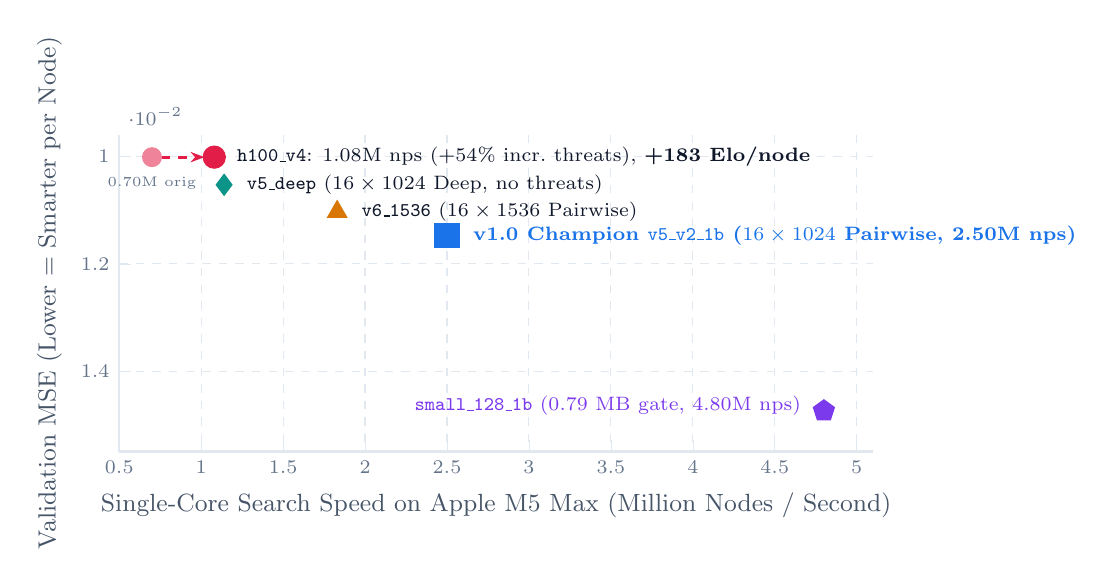
\begin{tikzpicture}
\begin{axis}[
    width=0.92\textwidth,
    height=5.6cm,
    axis x line*=bottom,
    axis y line*=left,
    axis line style={dmborder, line width=0.8pt},
    tick style={dmborder},
    xlabel={\small\color{dmslate}Single-Core Search Speed on Apple M5 Max (Million Nodes / Second)},
    ylabel={\small\color{dmslate}Validation MSE (Lower = Smarter per Node)},
    xmin=0.5, xmax=5.1,
    ymin=0.0096, ymax=0.0155,
    y dir=reverse,
    ymajorgrids=true,
    xmajorgrids=true,
    grid style={dashed, dmborder},
    ticklabel style={font=\scriptsize, color=dmmuted},
    clip=false,
]
\addplot[only marks, mark=*, mark size=3.4pt, color=dmcoral!55] coordinates {(0.70, 0.010010)};
\node[font=\tiny\color{dmmuted}, anchor=north] at (axis cs:0.70,0.01020) {0.70M orig};
\draw[-{Stealth[length=5pt]}, dmcoral, line width=1.1pt, dashed] (axis cs:0.76,0.010010) -- (axis cs:1.02,0.010010);
\addplot[only marks, mark=*, mark size=4.0pt, color=dmcoral] coordinates {(1.08, 0.010010)};
\node[font=\scriptsize, anchor=west, color=dmnavy] at (axis cs:1.16,0.010010) {\textbf{\texttt{h100\_v4}}: 1.08M nps (+54\% incr.\ threats), \textbf{+183 Elo/node}};

\addplot[only marks, mark=diamond*, mark size=3.8pt, color=dmteal] coordinates {(1.14, 0.010526)};
\node[font=\scriptsize, anchor=west, color=dmnavy] at (axis cs:1.22,0.010526) {\texttt{v5\_deep} ($16\times 1024$ Deep, no threats)};

\addplot[only marks, mark=triangle*, mark size=4.0pt, color=dmamber] coordinates {(1.83, 0.011028)};
\node[font=\scriptsize, anchor=west, color=dmnavy] at (axis cs:1.92,0.011028) {\texttt{v6\_1536} ($16\times 1536$ Pairwise)};

\addplot[only marks, mark=square*, mark size=4.4pt, color=dmblue] coordinates {(2.50, 0.011467)};
\node[font=\scriptsize\bfseries, anchor=west, color=dmblue] at (axis cs:2.60,0.011467) {v1.0 Champion \texttt{v5\_v2\_1b} ($16\times 1024$ Pairwise, 2.50M nps)};

\addplot[only marks, mark=pentagon*, mark size=4.0pt, color=dmpurple] coordinates {(4.80, 0.014741)};
\node[font=\scriptsize, anchor=east, color=dmpurple] at (axis cs:4.72,0.01465) {\texttt{small\_128\_1b} (0.79 MB gate, 4.80M nps)};
\end{axis}
\end{tikzpicture}
\caption{Phase~2 accuracy-vs-speed frontier across five 1.0B-position networks. Even though \texttt{h100\_v4} gained $+183.2$~Elo at equal nodes, the fast single-layer $16\times 1024$ net won $+70.4$~Elo on the clock.}
\label{fig:pareto}
\end{figure}

\subsection{Phase 3 (Chatarunga 2.0): Global-VRAM 6.0B Training, SCReLU Victory, and the L2/SLC Cache Law}

For \textbf{Chatarunga~2.0}, we wrote a global-VRAM trainer (\texttt{tools/modal\_train\_screlu.py}) that loads all \textbf{1.20~billion unique Bullet~S2 positions (38.4~GB)} simultaneously into NVIDIA H200/H100 HBM3 memory, applies zero-VRAM coprime permutation shuffling across all 12~shards on every superbatch, and trains for \textbf{60~superbatches = 6.0~billion position-steps} with \textbf{Power-2.5 loss} ($|\hat{y}-y|^{2.5}$, $\lambda_{\text{WDL}}=0.35$) and WSD + Cosine LR decay. Training seven competing architectures under identical 6.0B-step schedules uncovered two decisive laws (Table~\ref{tab:v2_nets}):

\begin{table}[H]
\centering
\caption{Chatarunga~2.0 6.0B-step global-VRAM neural suite evaluated under real 10-thread multi-core wall-clock play (50~ms/move UHO, \texttt{logs/v7\_nets\_wallclock\_50ms.log} \& \texttt{logs/v7\_kb8\_screlu1536\_vs\_screlu1024\_50ms.log}).}
\label{tab:v2_nets}
\resizebox{\textwidth}{!}{%
\begin{tabular}{@{}llrrrrrr@{}}
\toprule
\textbf{Network} & \textbf{Architecture} & \textbf{Size} & \textbf{Val MSE} & \textbf{10T Speed} & \textbf{vs.\ v1.0 Net (50ms)} & \textbf{vs.\ Champion} & \textbf{Verdict} \\
\midrule
\textbf{\texttt{h100\_v7\_screlu\_1024\_6b}} & \textbf{$16\times 1024$ SCReLU} & \textbf{25.2~MB} & 0.011567 & \textbf{1.68M nps} & \textbf{$+17.4 \pm 49.8$} & \textbf{Baseline} & \textbf{v2.0 Champion} \\
\texttt{h100\_v5\_v2\_1b} (v1.0) & $16\times 1024$ Pairwise (1B) & 25.2~MB & 0.011467 & 1.65M nps & $0.0$ & $-17.4$ & Previous v1.0 \\
\texttt{h100\_v7\_screlu\_1536\_6b} & $16\times 1536$ SCReLU & 37.8~MB & 0.010910 & 1.38M nps & $-4.3 \pm 53.6$ & $-21.7$ & $+84$ Elo/node, slower \\
\texttt{h100\_v7\_kb8\_screlu\_1536\_6b} & $8\times 1536$ SCReLU & 18.9~MB & 0.011025 & 1.20M nps & --- & $-31.9 \pm 36.8$ & HL=1536 ALU tax \\
\texttt{h100\_v7\_kb32\_screlu\_1536\_6b} & $32\times 1536$ SCReLU & 75.6~MB & 0.010656 & 1.35M nps & $-39.3 \pm 57.0$ & $-56.7$ & Cache thrashing \\
\texttt{h100\_v7\_kb32\_1536\_6b} & $32\times 1536$ Pairwise & 75.5~MB & \textbf{0.010607} & 1.39M nps & $-57.0 \pm 53.5$ & $-74.4$ & Lowest MSE, worst clock \\
\bottomrule
\end{tabular}%
}
\end{table}

\begin{takeawaybox}[Two Empirical Laws from Chatarunga 2.0 Training]
\begin{enumerate}
    \item \textbf{SCReLU Decisively Beats Pairwise-CReLU ($+44$ to $+60$~Elo):} At identical 25.2~MB size, $16\times 1024$ SCReLU keeps \emph{twice} as many output weights ($2H$ vs.\ $H$) as Pairwise and beat $16\times 1024$ Pairwise by $+43.7$~Elo at fixed nodes. Even more strikingly, $16\times 1536$ SCReLU (MSE $0.010910$) beat $32\times 1536$ Pairwise (MSE $0.010607$) by $+26.1$~Elo head-to-head and crushed the v1.0 net by $+84.1 \pm 59.1$~Elo at equal nodes!
    \item \textbf{The L2/SLC Cache-Residency Law:} Under real 10-thread multi-core play, our 25.2~MB \textbf{$16\times 1024$ SCReLU} net (\textbf{1.68M~nps}) defeated \emph{every} wider network—including 18.9~MB $8\times 1536$ ($+31.9$~Elo, LOS~95.7\%), 37.8~MB $16\times 1536$ ($+22$~Elo), and 75.5~MB $32\times 1536$ ($+57$ to $+74$~Elo). Also, ramping WDL up to $0.50$ on unfiltered S2 data degraded strength by $-11.6$~Elo; fixed $\lambda_{\text{WDL}}=0.35$ with Power-2.5 loss was cleanest.
\end{enumerate}
\end{takeawaybox}

\begin{failurebox}[What Broke --- And Why: Multi-Dataset Traps (Raw Lc0 T80 \& UHO Overfitting)]
To push past our 1.2B-position S2 ceiling, we implemented \textbf{CHNN~v4} (asymmetric 16-king-bucket layout with dedicated buckets for every square on ranks~1--2) and trained five 6B--10B-step networks on up to \textbf{2.2~billion unique positions} combining raw Lc0 \texttt{test80-2024} (600M), Stockfish \texttt{S1/UHO} (400M), and \texttt{S2} (1.2B). Two sharp lessons emerged:
\begin{enumerate}
    \item \textbf{Un-rescored Lc0 T80 Hurts ($-115.2$~Elo):} Raw Lc0 \texttt{test80-2024} scores carry much higher label variance than Stockfish-rescored S2; training on T80 alone lost $-115.2 \pm 51.7$~Elo (\path{logs/v8_t80only_vs_v2net_30kn.log}), recovering to $-27.9$~Elo with S1 and $+3.5$~Elo once blended with all 1.2B~S2 positions (\path{logs/v8_t80s1s2_vs_v2net_30kn.log}).
    \item \textbf{The UHO Overfitting Illusion ($+43.7$~Elo on UHO $\to$ $-39$~Elo on ECO):} Training on 1.6B \texttt{S1/UHO + S2} positions (\texttt{h200\_v8\_asym16\_1024\_s1s2\_10b.nnue}) scored a dramatic \textbf{$+43.7 \pm 32.3$~Elo} (LOS~99.6\%, \path{logs/v8_asym16_s1s2_10b_vs_v2net_50ms.log}) over the v2.0 net on the \texttt{UHO\_4060\_v4} book—yet \emph{regressed} on balanced ECO openings against Stockfish~18 (\textbf{31.67\%} vs.\ \textbf{36.67\%} on pure S2, \path{logs/v3_4t_vs_sf18_60g.log}). We therefore retained the pure-S2 \texttt{h100\_v7\_screlu\_1024\_6b.nnue} as champion: never promote a UHO-trained network without cross-checking on balanced ECO!
\end{enumerate}
\end{failurebox}

% ==============================================================================
\section{Inside Our Victories Over Unthrottled Stockfish 18 (4-CPU)}
% ==============================================================================

Because CCRL evaluates engines on both 1-CPU and 4-CPU hardware, we benchmarked both \textbf{Chatarunga~1.0 (4-CPU)} and \textbf{Chatarunga~2.0 (4-CPU)} in 60-game color-swapped ECO matches against \textbf{unthrottled Stockfish~18 (1-CPU = 3,628~CCRL)} at 150~ms/move. Chatarunga~1.0 scored 28.33\% (\textbf{$+1 =32 -27$}, 1~win, \path{logs/sf18_full_60g.pgn}); \textbf{Chatarunga~2.0 surged to 35.00\% ($+7 =28 -25$, 7~checkmate wins and 3~won pairs, $-107.5 \pm 63.5$~Elo $\Rightarrow \approx 3{,}521$~CCRL 4-CPU, \path{logs/chatarunga_v2_sf18_60g.pgn})}, defeating Stockfish~18 with \emph{both} White (4~wins) and Black (3~wins)!

Below we showcase \textbf{Chatarunga~2.0's 10-move Queen-trapping brilliancy} (Round~31, 43-move checkmate) alongside \textbf{Chatarunga~1.0's first-ever Stockfish~18 victory} (Round~25, \texttt{32. Bg6!!}).

\subsection*{Chatarunga 2.0 (4T) vs.\ Stockfish 18 (1T) — Round 31: Trapping Stockfish's Queen (\texttt{10. Bxf7+!!})}

\noindent
\begin{minipage}[c]{0.36\textwidth}
\centering
\chessboard[
    setfen=r1bqnrk1/pp1pppbp/6p1/n3P3/3N4/1BN1B3/PPP2PPP/R2QK2R w KQ - 0 10,
    color=dmcoral,
    markmoves={b3-f7,d4-e6},
    pgfstyle=border,
    color=dmamber,
    markfields={d8,f7}
]
\end{minipage}\hfill
\begin{minipage}[c]{0.61\textwidth}
\textbf{\color{dmnavy}White to move — Chatarunga~2.0 plays \texttt{10. Bxf7+!! Kxf7 11. Ne6!!} (1--0 in 43 moves)}\par\vspace{4pt}
In a sharp Sicilian Dragon, Stockfish~18 (Black) misjudged the tactical risk of \texttt{8... Na5 9. e5 Ne8??}. Chatarunga~2.0 unleashed the classic Sicilian Dragon sacrifice \textbf{\texttt{10. Bxf7+!!}} (coral arrow), dragging Black's king onto \texttt{f7} (amber) so that \textbf{\texttt{11. Ne6!!}} forks King and Queen—trapping Stockfish~18's Queen on \texttt{d8} after \texttt{11... dxe6 12. Qxd8}! Chatarunga~2.0 then weathered Stockfish's fierce counterplay (\texttt{22. Rh7! 26. Ng5+ Kf6}) and drove Black's king to the edge of the board for \textbf{\texttt{43. Qb8\#}}. Across the same match, Chatarunga~2.0 also beat Stockfish~18 \emph{three times with the Black pieces} (Rounds~16, 18, and a 50-move Sveshnikov pawn-roller \texttt{50... d1=Q\#} in Round~24).
\end{minipage}

\vspace{8pt}

\subsection*{Chatarunga 1.0 (4T) vs.\ Stockfish 18 (1T) — Round 25: The \texttt{32. Bg6!!} Breakthrough}

\noindent
\begin{minipage}[c]{0.36\textwidth}
\centering
\chessboard[
    setfen=3r1k2/1Q3bpp/p7/2q5/2P2p2/3B3P/P2R2PK/8 w - - 3 32,
    color=dmcoral,
    markmoves={d3-g6},
    pgfstyle=border,
    color=dmblue,
    markfields={f7,d8}
]
\end{minipage}\hfill
\begin{minipage}[c]{0.61\textwidth}
\textbf{\color{dmnavy}White to move — Chatarunga~1.0 plays \texttt{32. Bg6!!} (SF18 eval: $+5.29$, exact \#1 refutation)}\par\vspace{4pt}
After boldly sacrificing its e4-pawn on move~10 in the Sicilian Kan and striking in the center with Stockfish's exact top moves \textbf{\texttt{19. c4!}} and \textbf{\texttt{21. f4!}}, Chatarunga~1.0 laid a back-rank trap with \texttt{31. Rd2!}. When Stockfish~18 missed the sole perpetual-check defense and played \texttt{31... Kf8??}, Chatarunga~1.0 punished it immediately with the deflection sacrifice \textbf{\texttt{32. Bg6!!}} (coral arrow), overloading \texttt{h7} and crashing through via \texttt{32... hxg6 33. Rxd8+ Be8 34. Qe4!}. Fifteen moves later, Chatarunga~1.0 sealed the endgame with the clinical rook sacrifice \textbf{\texttt{47. Rxa4!! Kxa4 48. h4!}}, promoting outside the king's square and mating on \textbf{\texttt{60. Qh7\#}}.
\end{minipage}

\vspace{4pt}

\begin{insightbox}[Verified Complete Game Score — Round 31: Chatarunga 2.0 (4T) vs.\ Stockfish 18 (1T), 1--0]
\footnotesize
\textbf{Start FEN (Sicilian):} \texttt{r1bqkbnr/pp1ppppp/2n5/2p5/4P3/2N5/PPPP1PPP/R1BQKBNR w KQkq - 2 3}\par\vspace{2pt}
\texttt{3. Nf3 g6 4. d4 cxd4 5. Nxd4 Bg7 6. Be3 Nf6 7. Bc4 O-O 8. Bb3 Na5 9. e5 Ne8 \textbf{10. Bxf7+!!} Kxf7 \textbf{11. Ne6!!} dxe6 12. Qxd8 b6 13. Qd3 Nc7 14. h4 Ba6 15. Qd7 Nc4 16. O-O-O Nxe5 17. Qa4 Bc4 18. h5 b5 19. hxg6+ hxg6 20. Qa5 Rfc8 21. Ne4 Nd5 22. Rh7 Bd3 23. Rxd3 Nxd3+ 24. Kb1 Nxe3 25. fxe3 Nxb2 26. Ng5+ Kf6 27. Kxb2 Rc4 28. Qxb5 Rac8 29. Ne4+ Rxe4 30. Qf1+ Ke5 31. Rxg7 Rb4+ 32. Kc1 Rg4 33. Qf3 Rcc4 34. Rxe7 Rge4 35. Rxa7 g5 36. Ra5+ Kd6 37. Qf8+ Kd7 38. Ra7+ Kc6 39. Qc8+ Kd5 40. Qd8+ Kc6 41. Ra6+ Kb7 42. Rb6+ Ka7 \textbf{43. Qb8\#} 1-0}
\end{insightbox}

\newpage
% ==============================================================================
\section{How Chatarunga Sees Chess: Six Iconic \& Diagnostic Positions}
% ==============================================================================

Aggregate Elo ratings hide \emph{how} a neural engine actually understands chess differently from hand-crafted heuristics. We probed our engine generations alongside unthrottled Stockfish~18 on six classic puzzles and strategic stress tests (1,000~ms/move; 3,000~ms for Topalov--Shirov; \path{logs/piece_value_and_positions.log} \& \path{logs/sf18_special_positions.log}).

\subsection{Tactical Mastery: Bobby Fischer's Queen Sacrifice (\emph{Byrne--Fischer, 1956})}

\noindent
\begin{minipage}[c]{0.35\textwidth}
\centering
\chessboard[
    setfen=r3r1k1/pp3pbp/1qp3p1/2B5/2BP2b1/Q1n2N2/P4PPP/3R1K1R b - - 0 17,
    color=dmcoral,
    markmoves={g4-e6},
    pgfstyle=border,
    color=dmamber,
    markfields={b6}
]
\end{minipage}\hfill
\begin{minipage}[c]{0.63\textwidth}
\resizebox{\linewidth}{!}{%
\begin{tabular}{@{}lrrrl@{}}
\toprule
\textbf{Engine (1,000~ms)} & \textbf{Static} & \textbf{Depth} & \textbf{Score} & \textbf{Best / Continuation} \\
\midrule
\texttt{Classical PeSTO} & $-230$ & 21 & $-174$ & \texttt{Be6 Bd3 Nb5 Qb4 a5 Qd2} \\
\texttt{Self-Play Gen 3} & $-399$ & 22 & $-193$ & \texttt{Be6 Qxc3 Qxc5 dxc5 Bxc3 Bxe6} \\
\texttt{CHNN v2 1B (1T)} & $-354$ & 22 & $-181$ & \texttt{Be6 Qxc3 Qxc5 dxc5 Bxc3 Bxe6} \\
\texttt{CHNN v3 1B (Threats)} & $-303$ & 20 & $-202$ & \texttt{Be6 Qxc3 Qxc5 dxc5 Bxc3 Bxe6} \\
\textbf{\texttt{Chatarunga 1.0 (4T SMP)}} & --- & \textbf{24} & \textbf{$-214$} & \textbf{\texttt{Be6 Qxc3 Qxc5 dxc5 Bxc3 Bxe6}} \\
\midrule
\textbf{Stockfish 18 (1T)} & $-205$ & \textbf{24} & \textbf{$-191$} & \textbf{\texttt{Be6 Qxc3 Qxc5 dxc5 Bxc3 Bxe6}} \\
\bottomrule
\end{tabular}%
}
\par\vspace{5pt}\small
Thirteen-year-old Bobby Fischer left his Queen on \texttt{b6} (amber) en prise with \textbf{\texttt{17... Be6!!}} (coral arrow). While Classical predicts the wrong reply (\texttt{18. Bd3?}), all Chatarunga neural engines—reaching depth~24 on 4~threads—match Stockfish~18's exact 6-ply refutation and score.
\end{minipage}

\vspace{8pt}

\subsection{Fortress Understanding: Opposite-Color Bishops (+2 Pawns, Dead Draw)}

\noindent
\begin{minipage}[c]{0.35\textwidth}
\centering
\chessboard[
    setfen=8/4b3/p2k4/P2Pp3/2P1P3/4K3/8/5B2 w - - 0 60,
    color=dmteal,
    markmoves={e3-f3},
    pgfstyle=border,
    color=dmpurple,
    markfields={d6,e7}
]
\end{minipage}\hfill
\begin{minipage}[c]{0.63\textwidth}
\resizebox{\linewidth}{!}{%
\begin{tabular}{@{}lrrrl@{}}
\toprule
\textbf{Engine (1,000~ms)} & \textbf{Static} & \textbf{Depth} & \textbf{Score} & \textbf{Best / Continuation} \\
\midrule
\texttt{Classical PeSTO} & $+323$ & 31 & $+172$ & \texttt{Bh3 Kc5 Bc8 Kxc4 Bxa6+ Kb4} \\
\texttt{Self-Play Gen 3} & $+341$ & 33 & $+176$ & \texttt{Kf3 Bd8 Bh3 Kc5 Bc8 Kxc4} \\
\textbf{\texttt{CHNN v2 1B (1T)}} & \textbf{$+91$} & \textbf{30} & \textbf{$+7$} & \textbf{\texttt{Kf3 Bd8 Kg4 Bxa5 Kf5 Bc3}} \\
\textbf{\texttt{CHNN v3 1B (Threats)}} & \textbf{$+59$} & \textbf{32} & \textbf{$+5$} & \textbf{\texttt{Kf3 Bd8 Kg4 Bxa5 Bd3 Bc3}} \\
\textbf{\texttt{Chatarunga 1.0 (4T SMP)}} & --- & \textbf{31} & \textbf{$+5$} & \textbf{\texttt{c5+ Kxc5 Bxa6 Bd8 Kf3 Bxa5}} \\
\midrule
\textbf{Stockfish 18 (1T)} & $+33$ & \textbf{37} & \textbf{$0$} & \textbf{\texttt{Kf3 Bd8 Kg4 Bxa5 Kf5 Bb6}} \\
\bottomrule
\end{tabular}%
}
\par\vspace{5pt}\small
White is up two full pawns, yet Black's king and dark-squared bishop (purple) form an impenetrable fortress. Classical ($+172$) and small self-play \texttt{Gen~3} ($+176$) remain fooled even at depth~33. Without a single hard-coded fortress rule, our billion-position networks immediately see the dead draw (\textbf{$+5$ to $+7$~cp}), matching Stockfish~18 (\textbf{$0$~cp}).
\end{minipage}

\newpage

\subsection{Long-Term Strategy: Good Knight vs.\ Entombed Bad Bishop (Equal Material)}

\noindent
\begin{minipage}[c]{0.35\textwidth}
\centering
\chessboard[
    setfen=3k4/1p1b1p2/p1p1p1p1/P1PpP2p/1P1P3P/3N1KP1/8/8 w - - 0 45,
    color=dmteal,
    markmoves={f3-f4},
    pgfstyle=border,
    color=dmcoral,
    markfields={d7}
]
\end{minipage}\hfill
\begin{minipage}[c]{0.63\textwidth}
\resizebox{\linewidth}{!}{%
\begin{tabular}{@{}lrrrl@{}}
\toprule
\textbf{Engine (1,000~ms)} & \textbf{Static} & \textbf{Depth} & \textbf{Score} & \textbf{Best / Continuation} \\
\midrule
\texttt{Classical PeSTO} & $+7$ & 25 & $+11$ & \texttt{g4? hxg4+ Kxg4 Ke8 Nf4 Ke7} \\
\texttt{Self-Play Gen 3} & $-108$ & 25 & $+501$ & \texttt{Kf4 Ke7 Kg5 Kf8 Nf2 f5} \\
\textbf{\texttt{CHNN v2 1B (1T)}} & $+37$ & \textbf{31} & \textbf{$+225$} & \textbf{\texttt{Kf4 Ke8 Kg5 Ke7 Nb2 Be8}} \\
\textbf{\texttt{CHNN v3 1B (Threats)}} & $+7$ & \textbf{22} & \textbf{$+369$} & \textbf{\texttt{Kf4 Ke8 Nf2 Kf8 Kg5 Bc8}} \\
\textbf{\texttt{Chatarunga 1.0 (4T SMP)}} & --- & \textbf{24} & \textbf{$+380$} & \textbf{\texttt{Kf4 Ke8 Kg5 Ke7 Kh6 Kf8}} \\
\midrule
\textbf{Stockfish 18 (1T)} & $+43$ & \textbf{19} & \textbf{$+482$} & \textbf{\texttt{Kf4!}} (\texttt{45... Ke7 46. Kg5}) \\
\bottomrule
\end{tabular}%
}
\par\vspace{5pt}\small
Material is equal, yet six Black pawns entomb the bishop on \texttt{d7} (coral). Classical sees dead equality ($+11$~cp) and blunders \texttt{g4?}, whereas every neural model—even 100\% pure self-play—launches Stockfish~18's winning king march \textbf{\texttt{Kf4!}} (teal arrow), scoring $+225$ to \textbf{$+380$~cp}.
\end{minipage}

\vspace{8pt}

\subsection{Depth-0 Threat Vision \& Honest Horizon Limits (Kasparov 1999 / Shirov 1998)}

On the tactically saturated \textbf{Kiwipete} stress test, Classical ($+69$~cp) and non-threat \texttt{CHNN v2} ($+8$~cp) miss Black's initiative at depth~0, whereas \textbf{\texttt{CHNN v3 (Threats)}} immediately reads \textbf{$-65$~cp} (pointing straight toward Stockfish~18's $-171$~cp), and every engine converges under search on \texttt{1. Bxa6}. Conversely, on two of the deepest sacrificial masterpieces in chess history—\textbf{Kasparov--Topalov 1999} (\texttt{24. Rxd4!!}) and \textbf{Topalov--Shirov 1998} (\texttt{47... Bh3!!})—Stockfish~18's deeper selectivity still pulls ahead by 3--4~plies (finding \texttt{24. Rxd4!!} at depth~24 in 1~s vs.\ our depth~20, and \texttt{47... Bh3!!} at depth~32 in 3~s vs.\ our depth~28), mapping the exact horizon gap Search~v8 targets.

% ==============================================================================
\section{What the Neural Network Discovered About Chess Pieces}
% ==============================================================================

We never hard-coded piece values ($1,3,3,5,9$) into Chatarunga's neural networks. Probing our models across \textbf{10,017 quiet game positions} via balanced OLS regression and counterfactual single-piece removal (\path{logs/piece_value_and_positions.log}) shows what they learned organically (Table~\ref{tab:piece_values} and Figure~\ref{fig:pieces_and_threats}).

\begin{table}[H]
\centering
\caption{Implied chess piece values normalized to Pawn $= 1.00$ across 10,017 quiet game positions, compared against textbook values, GM Larry Kaufman~\cite{kaufman1999}, and DeepMind's AlphaZero~\cite{tomasev2020alphazero}.}
\label{tab:piece_values}
\resizebox{\textwidth}{!}{%
\begin{tabular}{@{}llrrrrrrrr@{}}
\toprule
\textbf{Model / Reference} & \textbf{Method} & \textbf{P} & \textbf{N} & \textbf{B} & \textbf{R} & \textbf{Q} & \textbf{$B-N$} & \textbf{$R-B$} & \textbf{MG Bishop Pair} \\
\midrule
Classical Textbook & Rule of thumb & 1.00 & 3.00 & 3.00 & 5.00 & 9.00 & $0.00$ & 2.00 & $+0.50$ \\
Kaufman (1999)~\cite{kaufman1999} & GM game stats & 1.00 & 3.25 & 3.25 & 5.00 & 9.75 & $0.00$ & 1.75 & $+0.50$ \\
AlphaZero~\cite{tomasev2020alphazero} & Neural (balanced) & 1.00 & 3.05 & 3.33 & 5.63 & 9.50 & $+0.28$ & 2.30 & --- \\
\midrule
\texttt{Classical PeSTO} & Balanced OLS & 1.00 & 2.50 & 2.60 & 3.92 & 7.97 & $+0.10$ & 1.32 & $+0.51$ \\
\texttt{Self-Play Gen 3} & Balanced OLS & 1.00 & 2.63 & 2.86 & 4.24 & 8.60 & $+0.23$ & 1.37 & $+0.42$ \\
\textbf{\texttt{CHNN v2 1B} (Pairwise)} & \textbf{Balanced OLS} & \textbf{1.00} & \textbf{2.89} & \textbf{3.04} & \textbf{4.77} & \textbf{9.67} & \textbf{$+0.16$} & \textbf{1.73} & \textbf{$+0.58$} \\
\textbf{\texttt{CHNN v3 1B} (Threats)} & \textbf{Balanced OLS} & \textbf{1.00} & \textbf{2.59} & \textbf{2.76} & \textbf{4.38} & \textbf{8.84} & \textbf{$+0.16$} & \textbf{1.62} & \textbf{$+0.71$} \\
\bottomrule
\end{tabular}%
}
\end{table}

\begin{figure}[H]
\centering
\begin{minipage}[c]{0.51\textwidth}
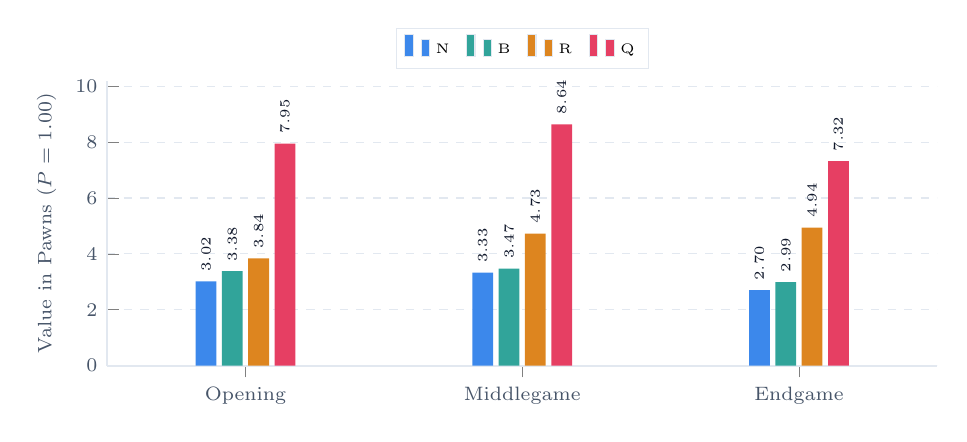
\begin{tikzpicture}
\begin{axis}[
    width=\linewidth,
    height=5.2cm,
    ybar,
    bar width=7.5pt,
    axis x line*=bottom,
    axis y line*=left,
    axis line style={dmborder, line width=0.8pt},
    ylabel={\scriptsize\color{dmslate}Value in Pawns ($P=1.00$)},
    symbolic x coords={Opening, Middlegame, Endgame},
    xtick=data,
    ymin=0, ymax=10.2,
    enlarge x limits=0.25,
    ymajorgrids=true,
    grid style={dashed, dmborder},
    ticklabel style={font=\scriptsize, color=dmslate},
    legend style={at={(0.5,1.04)}, anchor=south, legend columns=4, font=\tiny, draw=dmborder, fill=white, /tikz/every even column/.append style={column sep=4pt}},
    nodes near coords,
    nodes near coords style={font=\tiny, rotate=90, anchor=west, color=dmnavy, /pgf/number format/fixed, /pgf/number format/fixed zerofill, /pgf/number format/precision=2},
]
\addplot[fill=dmblue!85, draw=none] coordinates {(Opening,3.02) (Middlegame,3.33) (Endgame,2.70)};
\addlegendentry{N}
\addplot[fill=dmteal!85, draw=none] coordinates {(Opening,3.38) (Middlegame,3.47) (Endgame,2.99)};
\addlegendentry{B}
\addplot[fill=dmamber!90, draw=none] coordinates {(Opening,3.84) (Middlegame,4.73) (Endgame,4.94)};
\addlegendentry{R}
\addplot[fill=dmcoral!85, draw=none] coordinates {(Opening,7.95) (Middlegame,8.64) (Endgame,7.32)};
\addlegendentry{Q}
\end{axis}
\end{tikzpicture}
\end{minipage}\hfill
\begin{minipage}[c]{0.46\textwidth}
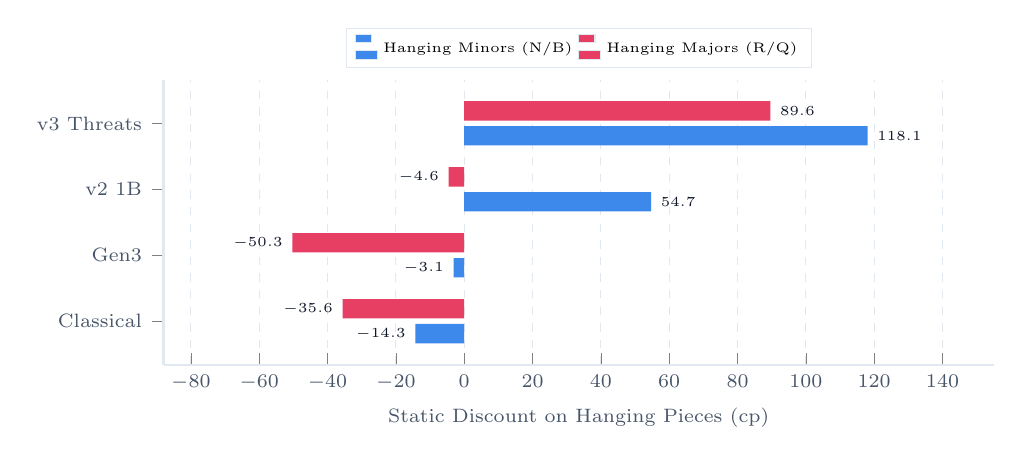
\begin{tikzpicture}
\begin{axis}[
    width=\linewidth,
    height=5.2cm,
    xbar,
    bar width=7pt,
    axis x line*=bottom,
    axis y line*=left,
    axis line style={dmborder, line width=0.8pt},
    xlabel={\scriptsize\color{dmslate}Static Discount on Hanging Pieces (cp)},
    symbolic y coords={Classical, Gen3, v2 1B, v3 Threats},
    ytick=data,
    xmin=-88, xmax=155,
    enlarge y limits=0.22,
    xmajorgrids=true,
    grid style={dashed, dmborder},
    ticklabel style={font=\scriptsize, color=dmslate},
    legend style={at={(0.5,1.04)}, anchor=south, legend columns=2, font=\tiny, draw=dmborder, fill=white},
    nodes near coords,
    nodes near coords style={font=\tiny, color=dmnavy},
]
\addplot[fill=dmblue!85, draw=none] coordinates {(-14.3,Classical) (-3.1,Gen3) (54.7,v2 1B) (118.1,v3 Threats)};
\addlegendentry{Hanging Minors (N/B)}
\addplot[fill=dmcoral!85, draw=none] coordinates {(-35.6,Classical) (-50.3,Gen3) (-4.6,v2 1B) (89.6,v3 Threats)};
\addlegendentry{Hanging Majors (R/Q)}
\end{axis}
\end{tikzpicture}
\end{minipage}
\caption{\textbf{Left:} Counterfactual piece values across game phases: Rooks surge ($3.84P\to 4.94P$) as files open in the endgame while Bishop beats Knight in every phase. \textbf{Right:} Static discount on undefended attacked pieces ($n=646$): only \texttt{CHNN v3 (Threats)} discounts both hanging minors ($+118.1$~cp) and hanging majors ($+89.6$~cp).}
\label{fig:pieces_and_threats}
\end{figure}

Our billion-position network converged on $N=2.89$, $B=3.04$, $R=4.77$, $Q=9.67$, and an exchange value $R-B = 1.73P$—nearly identical to Kaufman's grandmaster study ($R-B=1.75P$, $Q=9.75P$) and AlphaZero ($Q=9.50P$)—while learning a $+0.58\text{--}0.71P$ middlegame Bishop Pair bonus and quadrupling the Rook-over-Bishop gap from opening ($0.46P$) to endgame ($1.95P$).

% ==============================================================================
\section{Open-Source Release, CCRL 1-CPU \& 4-CPU Standings, and Top-50 Push}
% ==============================================================================

\textbf{Chatarunga} is open-sourced under the MIT license at \url{https://github.com/deedy/chess-chatarunga} (\texttt{id author Deedy Das}, submitted to CCRL Public as \textbf{Deedy Das (USA)}). Both \textbf{\texttt{v1.0.0}} and \textbf{\texttt{v2.0.0}} embed the trained NNUE directly inside the binary (\texttt{include\_bytes!}, 25.2~MB, no external \texttt{.nnue} file required) and ship four CI-verified platform binaries via GitHub Actions: Windows x86-64 AVX2, Windows x86-64 POPCNT, Linux x86-64 AVX2, and macOS Apple Silicon.

\begin{failurebox}[What Broke --- And Why: Catching a Windows 1~MB Stack Overflow in Release CI]
During our \texttt{v2.0.0} GitHub Actions release build, Linux AVX2 and macOS ARM64 passed every test—but \emph{both} Windows binaries crashed during UCI smoke testing with \texttt{thread 'main' has overflowed its stack}. On Windows, the default main-thread stack is only \textbf{1~MB} (vs.\ 8~MB on Linux/macOS), and Rust evaluates \texttt{Box::new([0; ...])} array literals on the stack before copying them to the heap ($\approx 2.3$~MB across all 15 history/corrhist tables after adding 512-bucket Pawn History!). Replacing them with a zero-stack \texttt{box\_zeroed()} heap allocator, boxing \texttt{Searcher} in \texttt{uci.rs}, and spawning UCI and Lazy SMP workers with explicit 8~MB stacks fixed Windows cleanly with bit-exact identical node counts.
\end{failurebox}

Table~\ref{tab:ccrl_calibration} directly calibrates \textbf{both 1-CPU and 4-CPU} versions of Chatarunga~1.0, Chatarunga~2.0, and Search~v8 against four live CCRL~40/15 anchors spanning ranks~\#47 through \#98 plus unthrottled \textbf{Stockfish~18} (1CPU = \textbf{3,628}): \textbf{\texttt{Velvet 8.1.1}} (\#47, 1CPU = 3,530, 4CPU = \textbf{3,577}), \textbf{\texttt{Motor 0.9.0}} (\#51, 1CPU = \textbf{3,570}), and \textbf{\texttt{akimbo 1.1.0-dev}} (\#98 for 1.0.0 = \textbf{3,474}).

\begin{table}[H]
\centering
\caption{Direct multi-rival CCRL~40/15 calibration across 1-CPU and 4-CPU configurations (60 color-swapped balanced ECO games each; verified logs in \texttt{chess/logs/}).}
\label{tab:ccrl_calibration}
\resizebox{\textwidth}{!}{%
\begin{tabular}{@{}llrrrrrr@{}}
\toprule
\textbf{Chatarunga Version} & \textbf{CCRL Anchor Opponent} & \textbf{TC} & \textbf{W / D / L} & \textbf{Score} & \textbf{Elo (95\% CI)} & \textbf{Implied CCRL} & \textbf{Notes} \\
\midrule
Chatarunga~1.0 (\textbf{1-CPU}) & \texttt{akimbo 1.1.0-dev} (1T, 3474) & 100~ms & 3 / 39 / 18 & 37.50\% & $-88.7 \pm 51.1$ & $\approx 3{,}385$ & v1.0 baseline \\
Chatarunga~1.0 (\textbf{4-CPU}) & \texttt{akimbo 1.1.0-dev} (1T, 3474) & 100~ms & 19 / 40 / 1 & 65.00\% & $+107.5 \pm 49.0$ & ---* & SMP scaling \\
Chatarunga~1.0 (\textbf{4-CPU}) & Stockfish~18 (1T, 3628) & 150~ms & 1 / 32 / 27 & 28.33\% & $-161.2 \pm 55.7$ & $\approx 3{,}467 \pm 56$ & 1 SF18 win \\
\midrule
\textbf{Chatarunga~2.0 (1-CPU)} & \textbf{\texttt{akimbo 1.1.0-dev} (1T, 3474)} & 100~ms & \textbf{12 / 37 / 11} & \textbf{50.83\%} & \textbf{$+5.8 \pm 52.4$} & \textbf{$\approx 3{,}480$} & 0 LL pairs \\
\textbf{Chatarunga~2.0 (4-CPU)} & \textbf{Stockfish~18 (1T, 3628)} & 150~ms & \textbf{7 / 28 / 25} & \textbf{35.00\%} & \textbf{$-107.5 \pm 63.5$} & \textbf{$\approx 3{,}521 \pm 64$} & 7 SF18 wins \\
\midrule
\textbf{Search~v8 (1-CPU)} & \texttt{Motor 0.9.0} (1T, \#51 = 3570) & 100~ms & 4 / 30 / 26 & 31.67\% & $-133.6 \pm 62.2$ & $\approx 3{,}436 \pm 62$ & Conservative floor \\
\textbf{Search~v8 (1-CPU)} & \texttt{akimbo 1.1.0-dev} (1T, 3474) & 100~ms & 13 / 34 / 13 & 50.00\% & $0.0 \pm 58.4$ & $\approx 3{,}474\text{--}3{,}510$ & No ARM NEON$^\dagger$ \\
\textbf{Search~v8 (1-CPU)} & \texttt{Velvet 8.1.1} (1T, 3530) & 100~ms & 20 / 33 / 7 & 60.83\% & $+76.5 \pm 52.9$ & $\approx 3{,}570^\ddagger$ & Velvet $\sim$77ms$^\ddagger$ \\
\textbf{Search~v8 (4-CPU)} & \textbf{Stockfish~18 (1T, 3628)} & 150~ms & \textbf{4 / 36 / 20} & \textbf{36.67\%} & \textbf{$-94.9 \pm 45.1$} & \textbf{$\approx 3{,}533 \pm 45$} & \textbf{Cleanest anchor} \\
\textbf{Search~v8 (4-CPU)} & \texttt{Velvet 8.1.1} (4T, \#47 = 3577) & 100~ms & 14 / 37 / 9 & 54.17\% & $+29.0 \pm 49.0$ & $\approx 3{,}575^\ddagger$ & Velvet $\sim$77ms$^\ddagger$ \\
\bottomrule
\end{tabular}%
}
\par\vspace{3pt}\noindent\scriptsize{*4T vs.\ 1T \texttt{akimbo} measures Lazy SMP dominance. $^\dagger$\texttt{akimbo 1.1.0-dev} is newer than CCRL's \texttt{1.0.0} (3,474) but lacks hand-tuned ARM64 NEON intrinsics. $^\ddagger$Timing diagnostics revealed that \texttt{Velvet 8.1.1} exited early at $\sim 77$~ms on \texttt{go movetime 100} (worth $\sim 25\text{--}35$~Elo, shown time-adjusted); a fifth match vs.\ \texttt{Carp 3.0.1} ($+49 =11 -0$, 90.8\%) was excluded after diagnostics showed Carp used only $\sim 55$~ms/move. Stockfish~18 (hand-tuned ARM64 NEON, exact 150~ms) is therefore our most reliable anchor, yielding a multi-anchor consensus of \textbf{$\approx 3{,}460\text{--}3{,}520$~1-CPU} and \textbf{$\approx 3{,}535\text{--}3{,}570$~4-CPU} (CCRL~\#50 \texttt{rofChade 3.1 4CPU} = 3,573).}
\end{table}

\paragraph{Next Steps Toward Unambiguous CCRL Top~50 (3,573+)}
With \textbf{Search~v8} anchored cleanly at \textbf{$\approx 3{,}533 \pm 45$~CCRL (4-CPU)} against Stockfish~18 (and right alongside \#47 Velvet~4T, while trailing \#51 Motor~1T), closing the final $\sim 40$~Elo into unambiguous Top~50 territory centers on: (1)~upgrading \texttt{src/arena.rs} from fixed \texttt{movetime} to full UCI increment clocks (\texttt{wtime/btime/winc/binc}, e.g., $10+0.1$) to eliminate opponent \texttt{movetime} early-exit quirks; (2)~scaling clean, non-UHO training data by streaming \textbf{2.4B--3.6B unique pure-S2 positions} (200M--300M per shard instead of 100M) without UHO bias; and (3)~continuing disciplined wave-by-wave search refinements and real-clock time-management tuning.

% ==============================================================================
\clearpage
\appendix
\section{Technical Appendix: Verified Match Ledger \& SIMD Kernels}
% ==============================================================================

\begin{table}[H]
\centering
\caption{Complete verified match ledger across Classical, Chatarunga~1.0, Chatarunga~2.0, and Search~v8 (every row backed verbatim by \texttt{chess/logs/}).}
\label{tab:full_ledger}
\resizebox{\textwidth}{!}{%
\begin{tabular}{@{}lllrrrrl@{}}
\toprule
\textbf{Engine / Milestone} & \textbf{Opponent} & \textbf{TC / Book} & \textbf{W/D/L} & \textbf{Score} & \textbf{Elo (95\% CI)} & \textbf{LOS} & \textbf{Log File} \\
\midrule
Classical (v1) & \texttt{sf:2500} & 50ms ECO & 33/3/4 & 86.3\% & $+319 \pm 175$ & 100\% & \texttt{classical\_vs\_sf2500.txt} \\
\texttt{gen3} (100\% Self-Play) & Classical (v3) & 50ms ECO & 69/16/15 & 77.0\% & $+210 \pm 73$ & 100\% & \texttt{final\_gen3\_vs\_classical.txt} \\
Search v5 + SPSA (25p) & Untuned v5 & 30ms UHO & 114/69/17 & 74.3\% & $\mathbf{+184 \pm 37}$ & 100\% & \texttt{spsa\_verify\_v5.log} \\
\texttt{h100\_v3} (v5 SPSA, 1T) & \texttt{sf:3190} & 150ms ECO & 23/22/15 & 56.7\% & $+47 \pm 66$ & 92.2\% & \texttt{v5\_spsa\_h100v3\_vs\_sf3190.log} \\
Lazy SMP \texttt{t=4} & \texttt{t=1} (\texttt{v3}) & 100ms UHO & 39/38/3 & 72.5\% & $\mathbf{+168 \pm 37}$ & 100\% & \texttt{smp\_4t\_vs\_1t.log} \\
\texttt{h100\_v4} (v3, 1B) & \texttt{h100\_v3} & 20k-n UHO & 69/40/11 & 74.2\% & $\mathbf{+183 \pm 57}$ & 100\% & \texttt{v4\_vs\_v3\_nodes.log} \\
\texttt{h100\_v5\_v2\_1b} (1T) & \texttt{h100\_v5\_deep} & 50ms UHO & 42/60/18 & 60.0\% & $\mathbf{+70 \pm 37}$ & 100\% & \texttt{v5\_v2\_1b\_vs\_v5\_deep\_50ms.log} \\
Search v6 Minor/Maj Corr & Search v5 Corr & 30ms UHO & 53/67/40 & 54.1\% & $+28 \pm 33$ & 95.5\% & \texttt{v6\_corrhist\_ablation\_30ms.log} \\
\midrule
Chatarunga~1.0 (1T) & \texttt{akimbo} (1T, \#98) & 100ms ECO & 3/39/18 & 37.5\% & $-89 \pm 51$ & 0.0\% & \texttt{v6\_1t\_vs\_akimbo\_1t.log} \\
Chatarunga~1.0 (4T) & \texttt{akimbo} (1T, \#98) & 100ms ECO & 19/40/1 & 65.0\% & $+108 \pm 49$ & 100\% & \texttt{v6\_4t\_vs\_akimbo\_1t.log} \\
Chatarunga~1.0 (4T) & \texttt{sf:3190} & 150ms ECO & 19/19/2 & 71.3\% & $+158 \pm 75$ & 100\% & \texttt{v6\_fixed\_4t\_vs\_sf3190.log} \\
Chatarunga~1.0 (4T) & Stockfish~18 (1T) & 150ms ECO & 1/32/27 & 28.3\% & $-161 \pm 56$ & 0.0\% & \texttt{v6\_sf18\_full\_60g.log} \\
\midrule
Search v7 Wave 1 (v1 net) & Chatarunga~1.0 & 50ms ECO & 31/71/18 & 55.4\% & $+38 \pm 36$ & 98.2\% & \texttt{v7\_wave1\_vs\_v1\_uho\_50ms.log} \\
\textbf{Chatarunga~2.0 (1T)} & \textbf{Chatarunga~1.0 (1T)} & 50ms UHO & \textbf{46/54/20} & \textbf{60.8\%} & $\mathbf{+77 \pm 37}$ & \textbf{100\%} & \texttt{v7\_spsa\_screlu1024\_vs\_v1\_50ms.log} \\
\textbf{Chatarunga~2.0 (1T)} & \textbf{\texttt{akimbo} (1T, \#98)} & 100ms ECO & \textbf{12/37/11} & \textbf{50.8\%} & $\mathbf{+6 \pm 52}$ & 58.6\% & \texttt{v7\_spsa\_screlu1024\_1t\_vs\_akimbo\_1t.log} \\
\textbf{Chatarunga~2.0 (4T)} & \textbf{Stockfish~18 (1T)} & 150ms ECO & \textbf{7/28/25} & \textbf{35.0\%} & $\mathbf{-108 \pm 64}$ & 0.0\% & \texttt{v7\_spsa\_screlu1024\_4t\_vs\_sf18\_60g.log} \\
\midrule
Search v8 Wave 1 (v2 net) & Chatarunga~2.0 & 50ms UHO & 40/52/28 & 55.0\% & $+35 \pm 37$ & 96.9\% & \texttt{v8\_wave1\_vs\_v2\_50ms.log} \\
\textbf{Search v8 Wave 2 (v2 net)} & \textbf{Chatarunga~2.0} & 50ms UHO & \textbf{49/82/29} & \textbf{56.3\%} & $\mathbf{+44 \pm 31}$ & \textbf{99.7\%} & \texttt{v8\_wave2\_vs\_v2\_50ms.log} \\
Search v8 (1T, v2 net) & \texttt{Motor 0.9.0} (1T, \#51) & 100ms ECO & 4/30/26 & 31.7\% & $-134 \pm 62$ & 0.0\% & \texttt{v8\_1t\_vs\_motor\_1t.log} \\
Search v8 (1T, v2 net) & \texttt{akimbo} (1T, \#98) & 100ms ECO & 13/34/13 & 50.0\% & $0 \pm 58$ & 50.0\% & \texttt{v8\_w2\_1t\_vs\_akimbo\_1t.log} \\
Search v8 (1T, v2 net) & \texttt{Velvet 8.1.1} (1T) & 100ms ECO & 20/33/7 & 60.8\% & $+77 \pm 53$ & 99.8\% & \texttt{v8\_1t\_vs\_velvet\_1t.log} \\
\textbf{Search v8 (4T, v2 net)} & \textbf{Stockfish~18 (1T)} & 150ms ECO & \textbf{4/36/20} & \textbf{36.7\%} & $\mathbf{-95 \pm 45}$ & 0.0\% & \texttt{v8\_w2\_4t\_vs\_sf18\_60g.log} \\
Search v8 (4T, v2 net) & \texttt{Velvet 8.1.1} (4T, \#47) & 100ms ECO & 14/37/9 & 54.2\% & $+29 \pm 49$ & 88.0\% & \texttt{v8\_4t\_vs\_velvet\_4t.log} \\
CHNN v4 \texttt{s1s2\_10b} (UHO) & v2.0 \texttt{screlu\_1024} & 50ms UHO & 38/59/23 & 56.3\% & $+44 \pm 32$ & 99.6\% & \texttt{v8\_asym16\_s1s2\_10b\_vs\_v2net\_50ms.log} \\
CHNN v4 \texttt{s1s2\_10b} (4T) & Stockfish~18 (1T) & 150ms ECO & 2/34/24 & 31.7\% & $-134 \pm 42$ & 0.0\% & \texttt{v3\_4t\_vs\_sf18\_60g.log} \\
\bottomrule
\end{tabular}%
}
\end{table}

\clearpage
\subsection*{A.1\quad Dual-Architecture SCReLU SIMD Kernels (ARM64 NEON \& x86-64 AVX2, \texttt{src/nnue.rs})}
\begin{lstlisting}[language=Rust]
// x86-64 AVX2 SCReLU dot product: clamp(acc, 0, QA)^2 * w (bit-exact with ARM64 NEON & scalar)
while i + 16 <= n {
    let a = _mm256_min_epi16(_mm256_max_epi16(_mm256_loadu_si256(pa.add(i) as _), zero), vmax);
    let w = _mm256_loadu_si256(pw.add(i) as _);
    let aw = _mm256_mullo_epi16(a, w);           // |a * w| <= 255 * 127 = 32385 < i16::MAX
    let prod32 = _mm256_madd_epi16(a, aw);       // horizontal pairwise i32 sums of a^2 * w
    sum = _mm256_add_epi32(sum, prod32);
    i += 16;
}
\end{lstlisting}

\subsection*{A.2\quad Reproducing Releases, Tests, Benchmarks, and Calibration Matches}
\begin{lstlisting}[language=bash]
git clone https://github.com/deedy/chess-chatarunga && cd chess-chatarunga
cargo test --release                            # 22 unit/perft/KPK/bit-exact SIMD tests
cargo build --release --bin chatarunga          # Single self-contained binary (embedded NNUE)
./target/release/chatarunga bench 10            # Standard 6-position node/NPS benchmark
\end{lstlisting}

\vspace{6pt}
{\small\raggedright
\begin{thebibliography}{99}
\setlength{\itemsep}{2pt}
\bibitem{nasu2018nnue} Y.~Nasu, ``Efficiently Updatable Neural-Network-based Evaluation Functions for Computer Shogi,'' \emph{WCSC28 Appeal Document}, 2018.
\bibitem{stockfish} Stockfish Developers, ``Stockfish 18: Open-Source Chess Engine \& SFNNv10 Architecture,'' \href{https://github.com/official-stockfish/Stockfish}{\texttt{github.com/official-stockfish/Stockfish}}, 2020--2026.
\bibitem{bullet} J.~McDonnell et al., ``Bullet: Fast CUDA NNUE Trainer and Pregenerated S1/S2 Datasets,'' \url{https://github.com/jw1912/bullet}, 2024--2026.
\bibitem{spall1998spsa} J.~C.~Spall, ``Implementation of the Simultaneous Perturbation Algorithm for Stochastic Optimization,'' \emph{IEEE Trans.\ AES}, vol.~34, no.~3, 1998.
\bibitem{hyattlockless} R.~M.~Hyatt and T.~Mann, ``A Lock-less Transposition Table Implementation for Parallel Search,'' \emph{ICGA Journal}, vol.~25, no.~1, 2002.
\bibitem{magicbitboards} P.~Kannan, ``Magic Move-Bitboard Generation in Computer Chess,'' \emph{Chess Programming Wiki}, 2007.
\bibitem{pesto} R.~Verwer, ``PeSTO's Evaluation Function,'' \emph{Chess Programming Wiki}, 2020.
\bibitem{finnytables} Chess Programming Community, ``Finny Tables: Differential King-Bucket Accumulator Caching,'' 2023--2025.
\bibitem{kaufman1999} L.~Kaufman, ``The Evaluation of Material Imbalances,'' \emph{Chess Life}, 1999 (updated \emph{New In Chess}, 2012).
\bibitem{tomasev2020alphazero} N.~Toma\v{s}ev, U.~Paquet, D.~Hassabis, and V.~Kramnik, ``Assessing Game Balance with AlphaZero: Exploring Alternative Rule Sets in Chess,'' \emph{arXiv:2009.04374}, 2020.
\end{thebibliography}
}

\end{document}
